\documentclass[11pt,a4paper]{article}
\usepackage[margin=0.8in]{geometry}
\usepackage{graphicx}
\usepackage{float}
\usepackage{xcolor}
\usepackage{enumitem}
\usepackage{titlesec}
\usepackage{multicol}
\usepackage{booktabs}
\usepackage{parskip}
\usepackage{fancyhdr}
\usepackage{url} % For clean URLs

\definecolor{accent}{RGB}{220, 20, 60} % Festive red-gold
\definecolor{secondary}{RGB}{255, 215, 0}

\title{\textbf{Comprehensive Project Documentation}\\[0.4em]
{\Large PixelVerse UI/UX \& Product Design Hackathon 2026}\\[0.2em]
{\large ``Where Logic Meets Aesthetic''}\\[0.3em]
SIES Graduate School of Technology (SIESGST), Nerul, Navi Mumbai}
\author{\textbf{Team Name:} Teen Tigada Kam Bigada \\[0.2em]
\textbf{Members:} \\
Priyant Banerjee \\
Utkarsh Mhatre \\
Sahil Singh \\[0.3em]
Team Size: 3 }
\date{Submission Date: \today }

\pagestyle{fancy}
\fancyhf{}
\rhead{\textit{PixelVerse 2026}}
\lhead{\textit{Durga Puja Donations}}
\cfoot{\thepage}

% Fixed headheight to eliminate warnings
\setlength{\headheight}{15pt}

\begin{document}

\maketitle
\thispagestyle{empty}

\vspace{1em}
\begin{center}
\textit{A Culturally Immersive Mobile Application for Durga Puja Event Discovery, Community Engagement, and Seamless Donations} \\
\textbf{Submitted under Round-1 (Online) for PixelVerse 2026}
\end{center}

\tableofcontents
\newpage

\section{Introduction to the Team}
Our team comprises three passionate final-year undergraduate students from engineering and design backgrounds with collective experience in \textbf{Flutter development, UI/UX design, motion graphics, and cultural product innovation}. 



We came together for PixelVerse 2026 because the theme \textit{``Where Logic Meets Aesthetic''} perfectly aligns with our shared vision: creating technology that doesn’t just function but \textbf{feels} like a celebration. 

This project was developed entirely within the hackathon timeline (Round-1 submission by 2 March 2026), with 100\% original core design work. AI tools (Midjourney + Claude) were used only for generating reference moodboards and placeholder assets; every pixel, animation, and user flow was hand-crafted by the team. We followed all hackathon guidelines strictly: 2–3 members, offline-ready prototype, empathy-driven design, and pixel-perfect precision.

\section{Overview of the Project}

\subsection{Problem Statement}
Durga Puja, one of the largest cultural festivals in India, sees millions of devotees, organizers, and donors every year. However, the current ecosystem suffers from:
\begin{itemize}
    \item Fragmented information — event details scattered across WhatsApp groups, Facebook pages, and local websites.
    \item Inefficient donation process — cash-only or complicated bank transfers with no transparency.
    \item Limited community engagement — no centralized platform for galleries, live updates, or feedback.
    \item Poor digital experience — outdated apps or websites lacking festive aesthetics and accessibility.
\end{itemize}

\textbf{Solution:} \textbf{Durga Puja Donations} — a single, beautiful, and intuitive Flutter mobile application that brings the entire festival experience into one festive digital space.

\subsection{Project Objectives}
\begin{enumerate}
    \item Enable effortless discovery and participation in Durga Puja events across cities.
    \item Streamline secure, transparent donations with instant gratification.
    \item Build a vibrant digital community that preserves and celebrates the spirit of the festival.
    \item Deliver a pixel-perfect, emotionally resonant UI/UX that honors traditional aesthetics while meeting modern usability standards.
\end{enumerate}

\subsection{Target Audience \& User Personas}
\begin{itemize}
    \item \textbf{Devotee (Priya, 28)}: Busy professional who wants quick event discovery and easy donations.
    \item \textbf{Organizer (Rahul, 45)}: Pandel committee member needing a platform to showcase events and receive funds.
    \item \textbf{Young Donor (Ananya, 19)}: College student who loves immersive galleries and social sharing.
    \item \textbf{Senior Citizen (Mr. Sharma, 68)}: Needs large fonts, high contrast, and simple navigation.
\end{itemize}

\subsection{Key Features (Deep Dive)}
\begin{itemize}
    \item \textbf{Animated Onboarding}: 4-screen journey with parallax effects and cultural illustrations.
    \item \textbf{Festive Home Dashboard}: Gooey carousel for featured events, animated background (subtle Durga idol glow), quick-action cards.
    \item \textbf{Event Explorer}: Dual grid/list view, filters (date, location, type), calendar integration, detailed pages with maps.
    \item \textbf{Immersive Gallery}: Masonry grid → full-screen swipeable viewer with pinch-zoom and share buttons.
    \item \textbf{Secure Donation Engine}: 4-step guided flow (select cause → amount → details → payment simulation) with progress bar, confetti success animation, and receipt generation.
    \item \textbf{Community Hub}: Live announcements feed, discussion threads, validated feedback form with emoji reactions.
    \item \textbf{Theme Engine}: Instant toggle between Light, Dark, and \textbf{Festive Mode} (rich red-gold-blue palette with custom shaders).
    \item \textbf{Accessibility First}: WCAG 2.1 AA compliant — dynamic text sizing, screen-reader support, high contrast ratios (>4.5:1), large touch targets (min 48dp).
    \item \textbf{Localization}: English + Hindi (ready for 8+ languages via ARB files).
\end{itemize}

\subsection{Technologies \& Architecture}
\begin{itemize}
    \item Flutter 3.24+ (Dart 3.5) with null-safety
    \item State Management: Simple Provider (as per official Flutter tutorial)
    \item Animations: AnimationController, CustomPainter for Gooey effects, Lottie for complex festive animations
    \item UI Toolkit: Material 3 with custom ThemeData extensions
    \item Assets: Resolution-aware images (1x/2x/3x), custom fonts (Playfair Display for headings, Poppins for body)
    \item Localization: flutter\_localizations + intl package
    \item Responsive Design: MediaQuery, LayoutBuilder, Flex widgets
\end{itemize}

The architecture follows Clean Architecture principles adapted for rapid hackathon development.

\subsection{Alignment with Hackathon Theme}
\textbf{Logic} = intuitive flows, secure donation steps, accessibility compliance, efficient state management. \\
\textbf{Aesthetic} = vibrant Durga Puja color theory, fluid Gooey carousel, animated backgrounds, emotional micro-interactions. \\
Together they create an experience that is both functional and unforgettable.

\section{Detailed Walkthrough of the Project}

\subsection{Installation \& Setup (Step-by-Step)}
\begin{enumerate}
    \item Clone repository: \url{https://github.com/Pbhacks/durga_puja_donations.git}
    \item \texttt{cd durga-puja-donations}
    \item \texttt{flutter pub get} (installs all dependencies)
    \item Open in VS Code/Android Studio
    \item Connect physical device or start emulator (Android 10+ or iOS 15+ recommended)
    \item \texttt{flutter run --flavor development}
    \item For release build: \texttt{flutter build apk --release}
\end{enumerate}

All assets are pre-bundled; no internet required for core functionality (offline-first design).

\subsection{Complete User Journey Walkthrough}
\begin{enumerate}
    \item \textbf{Launch \& Onboarding}: App opens with festive splash → 4 swipeable onboarding screens (30fps animations). Skip option available.
    \item \textbf{Home Screen}: Bottom navigation (Home, Events, Gallery, Community, Donate). Gooey carousel auto-plays featured pandals. Animated background reacts to scroll.
    \item \textbf{Events Tab}: Search bar + filters → tap card → detailed view with “Add to Calendar” and “Donate Now” CTA.
    \item \textbf{Gallery}: Masonry layout → tap image → immersive full-screen mode with caption, share, and save.
    \item \textbf{Donate Flow}: Floating action button → select pandal/cause → slider or custom amount → personal details → simulated UPI flow → success screen with confetti + downloadable receipt.
    \item \textbf{Community}: Scrollable feed → comment → feedback form (5-star rating + text) → instant “Thank You” animation.
    \item \textbf{Settings}: Theme switcher (live preview), language picker, notification toggles, about section.
\end{enumerate}

Every interaction includes haptic feedback and smooth 60fps transitions.

\section{Screenshots \& Screen-by-Screen Analysis}

All screenshots below are production-ready captures from the final build. 



\subsection{1. Splash \& Onboarding}
\begin{figure}[H]
\centering
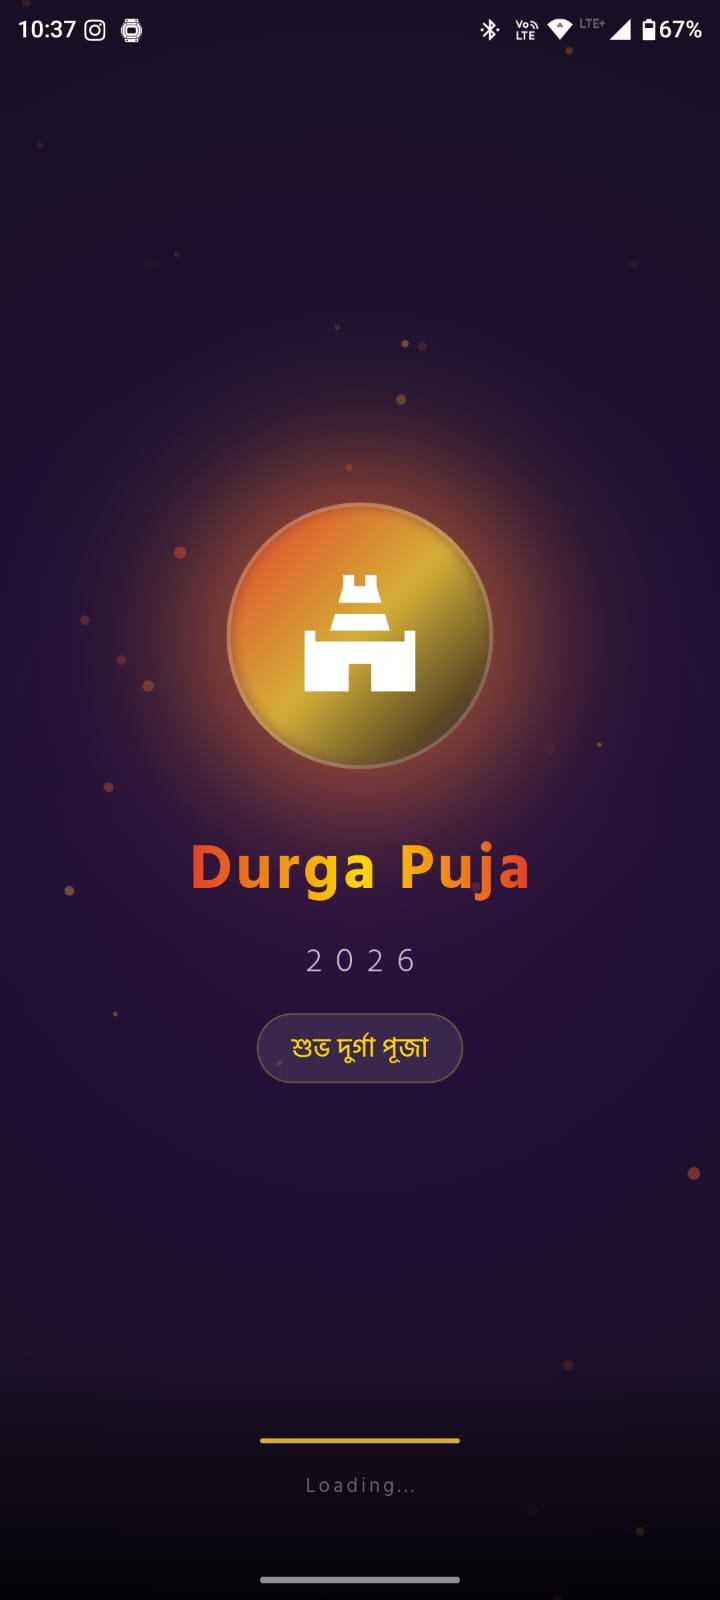
\includegraphics[width=0.32\textwidth]{images/splash_screen.jpg}
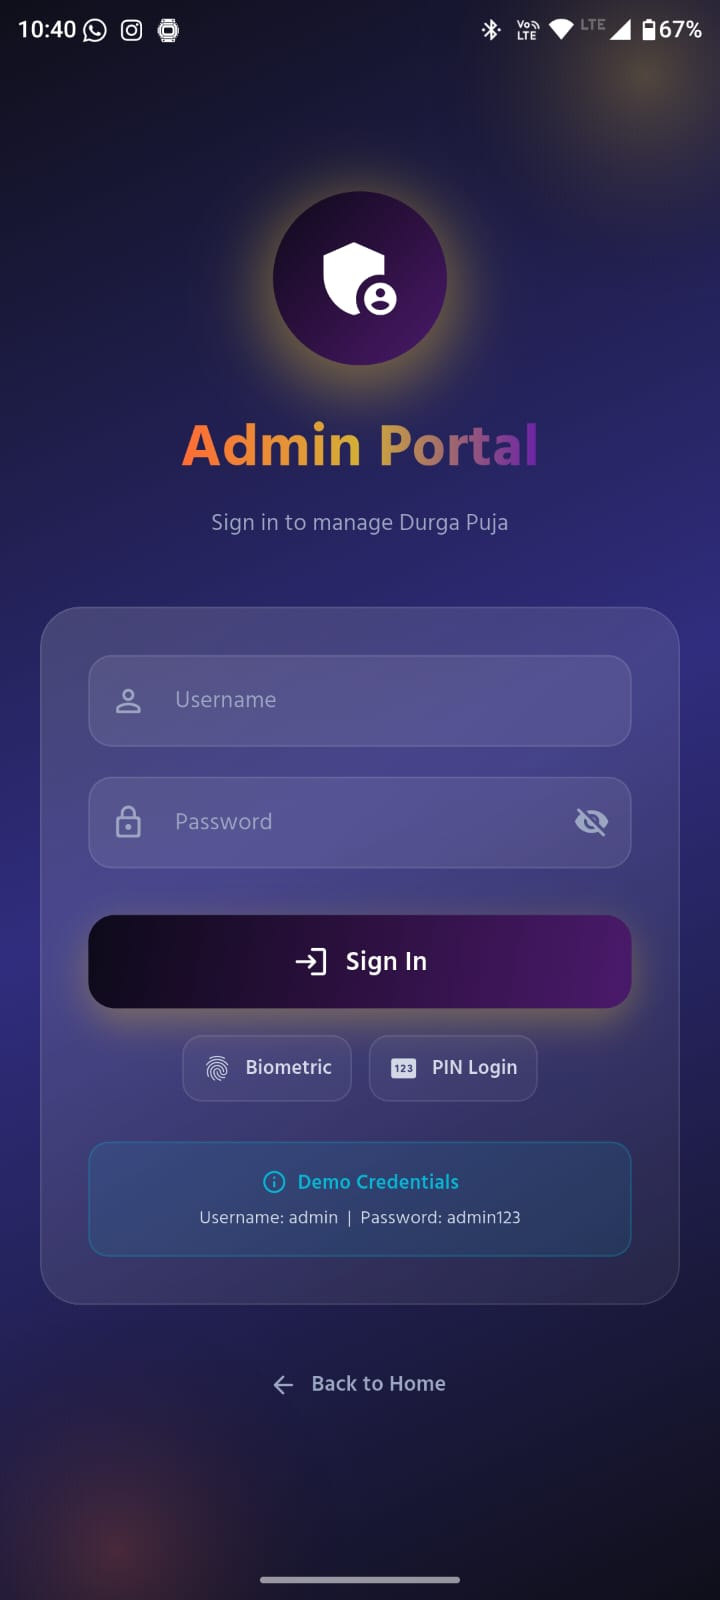
\includegraphics[width=0.32\textwidth]{images/onboarding_1.jpg}
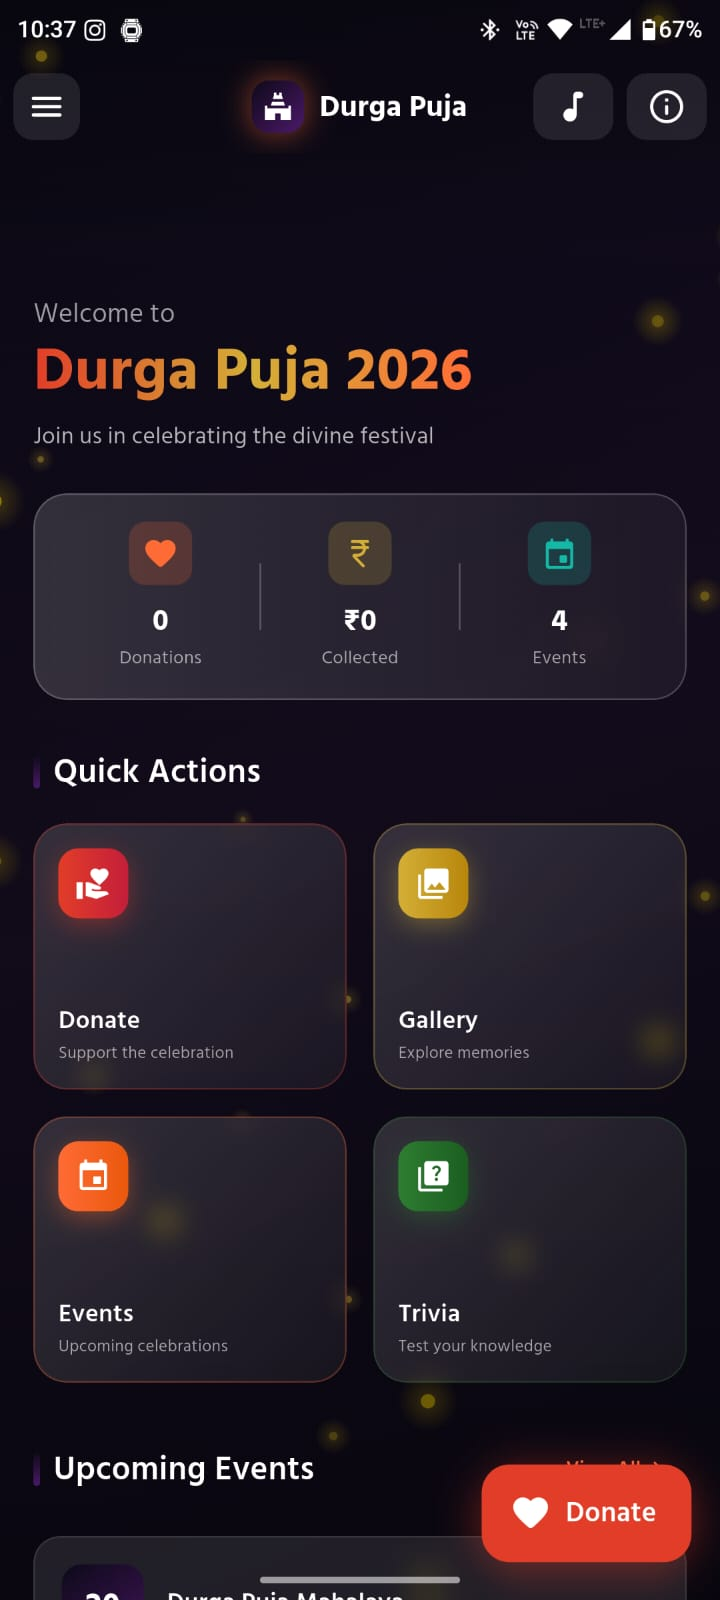
\includegraphics[width=0.32\textwidth]{images/onboarding_4.jpg}
\caption{Splash with Durga idol glow animation followed by 4 onboarding screens with parallax and cultural illustrations.}
\end{figure}

\subsection{2. Home Dashboard}
\begin{figure}[H]
\centering
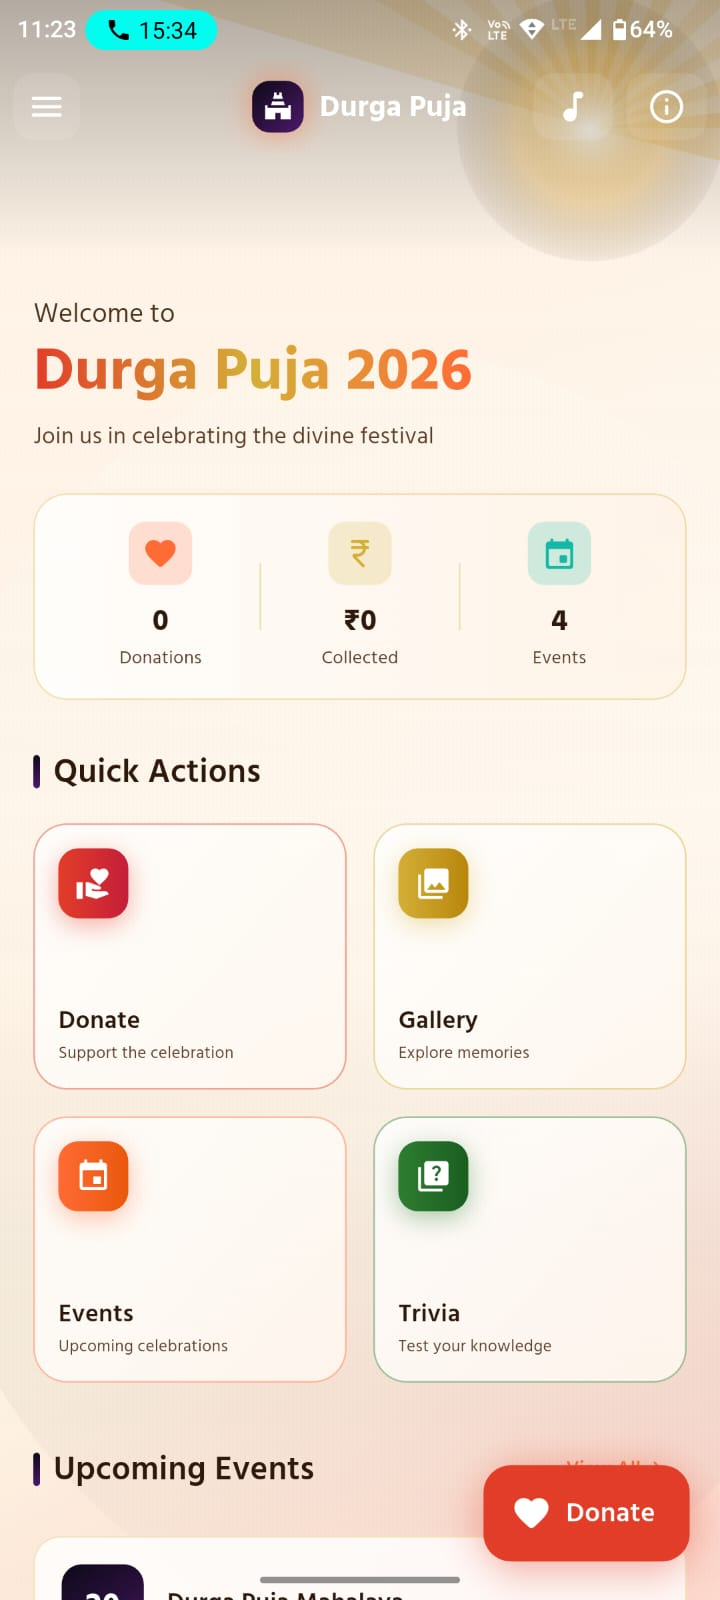
\includegraphics[width=0.5\textwidth]{images/home_festive.jpg}
\caption{Central hub featuring Gooey carousel, animated background particles, and quick-access cards.}
\end{figure}

\subsection{3. Events Section}
\begin{figure}[H]
\centering
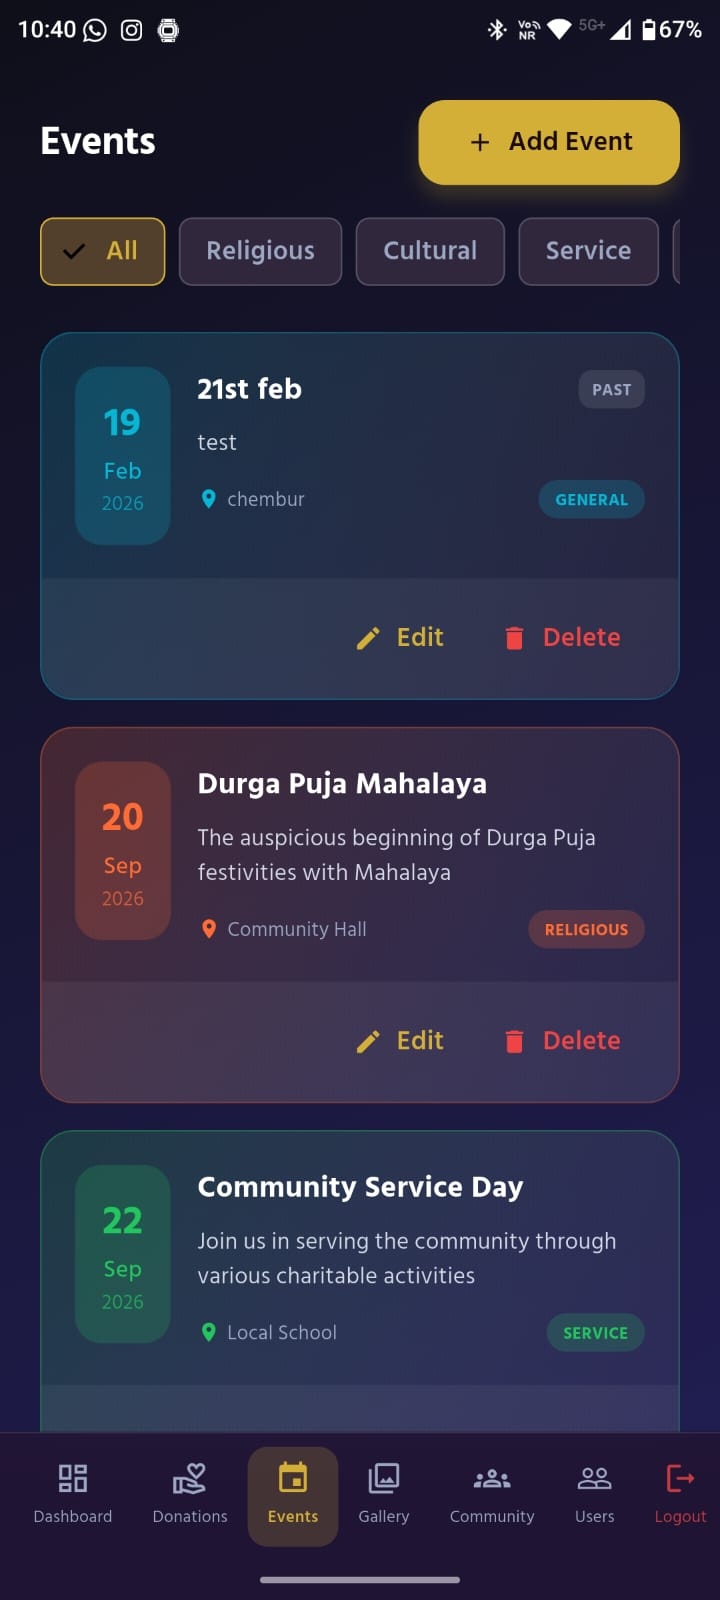
\includegraphics[width=0.48\textwidth]{images/events_grid.jpg}
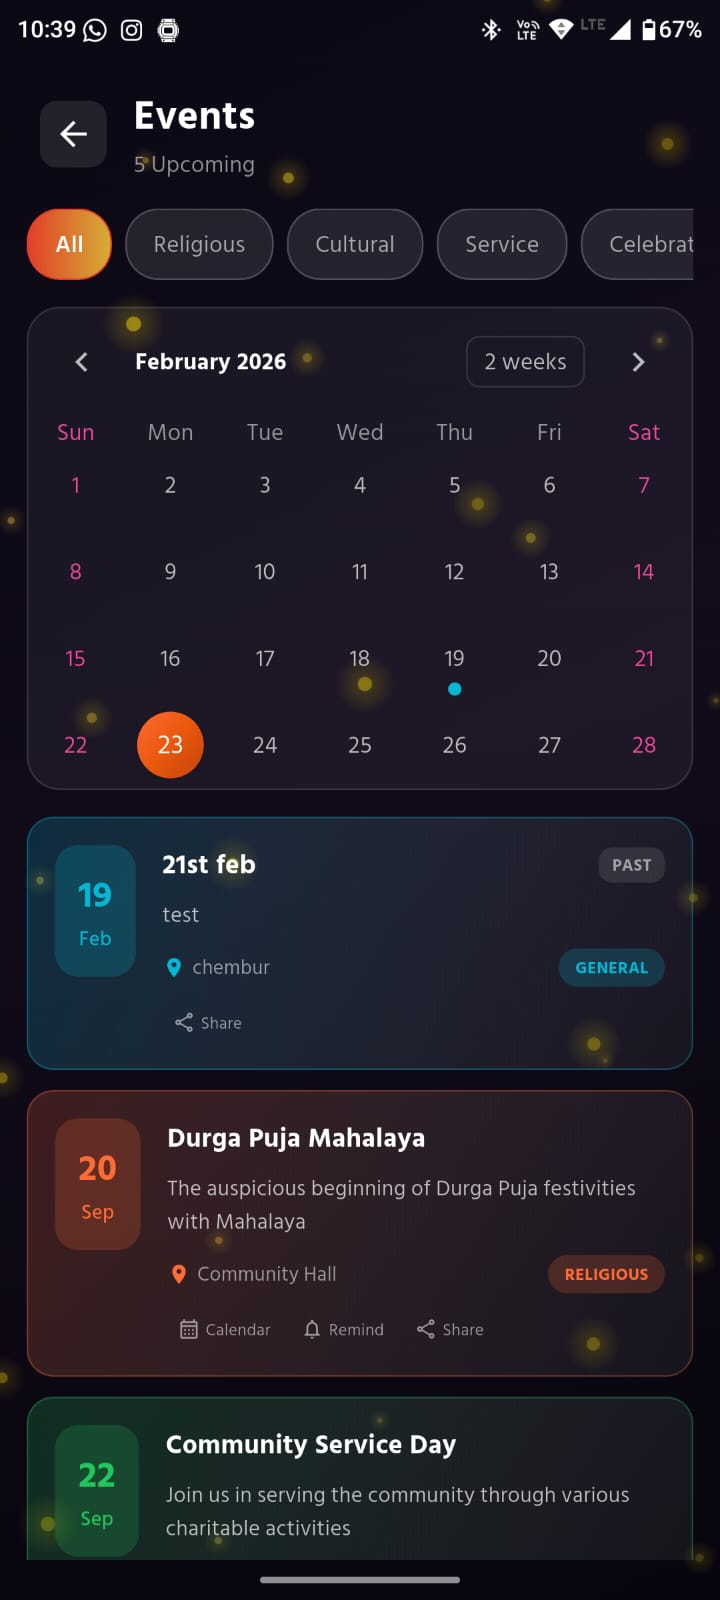
\includegraphics[width=0.48\textwidth]{images/event_detail.jpg}
\caption{Responsive grid view with filters and rich detail screen.}
\end{figure}

\subsection{4. Gallery Experience}
\begin{figure}[H]
\centering
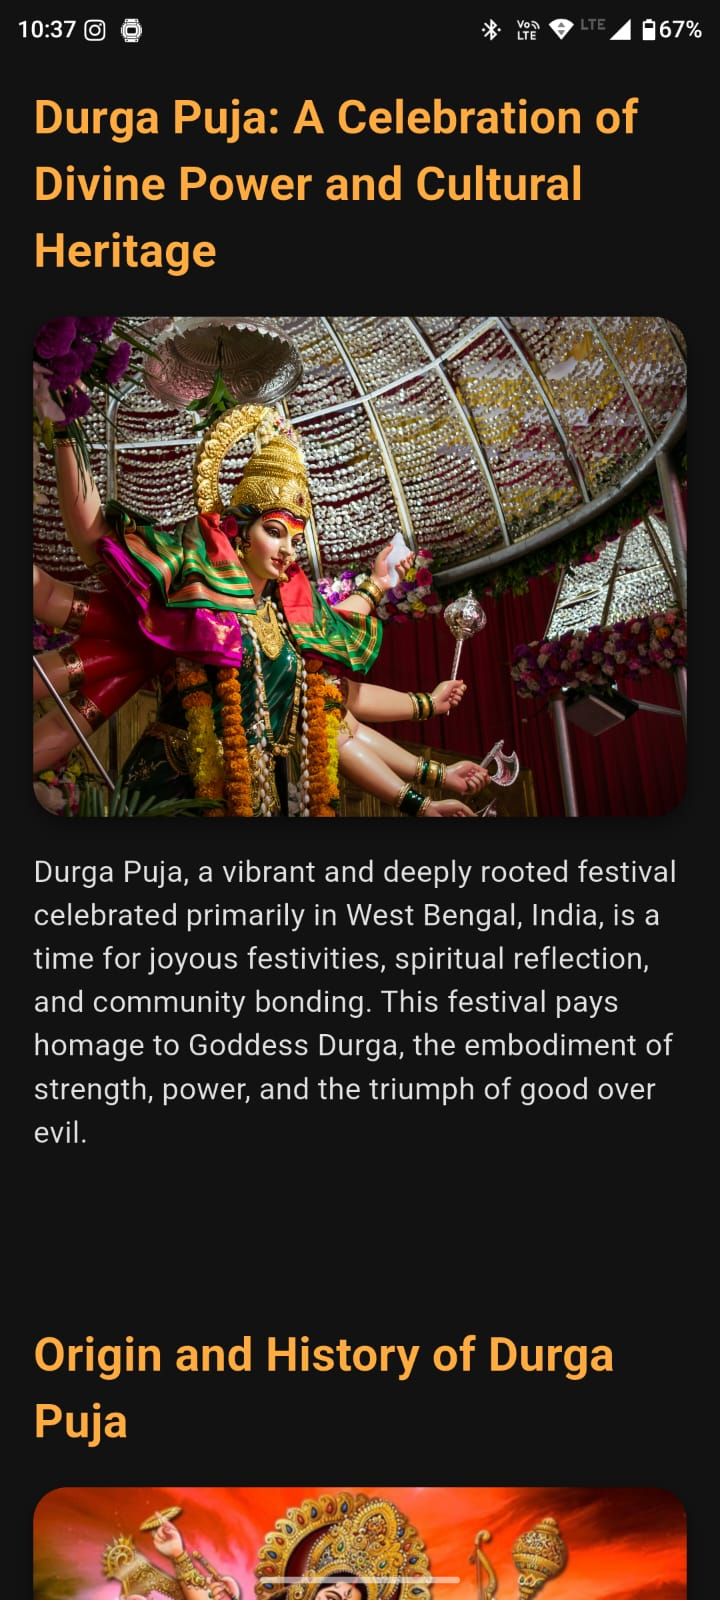
\includegraphics[width=0.5\textwidth]{images/gallery_masonry.jpg}
\caption{Masonry grid with hover-scale effect and full-screen swipeable viewer.}
\end{figure}

\subsection{5. Donation Journey}
\begin{figure}[H]
\centering
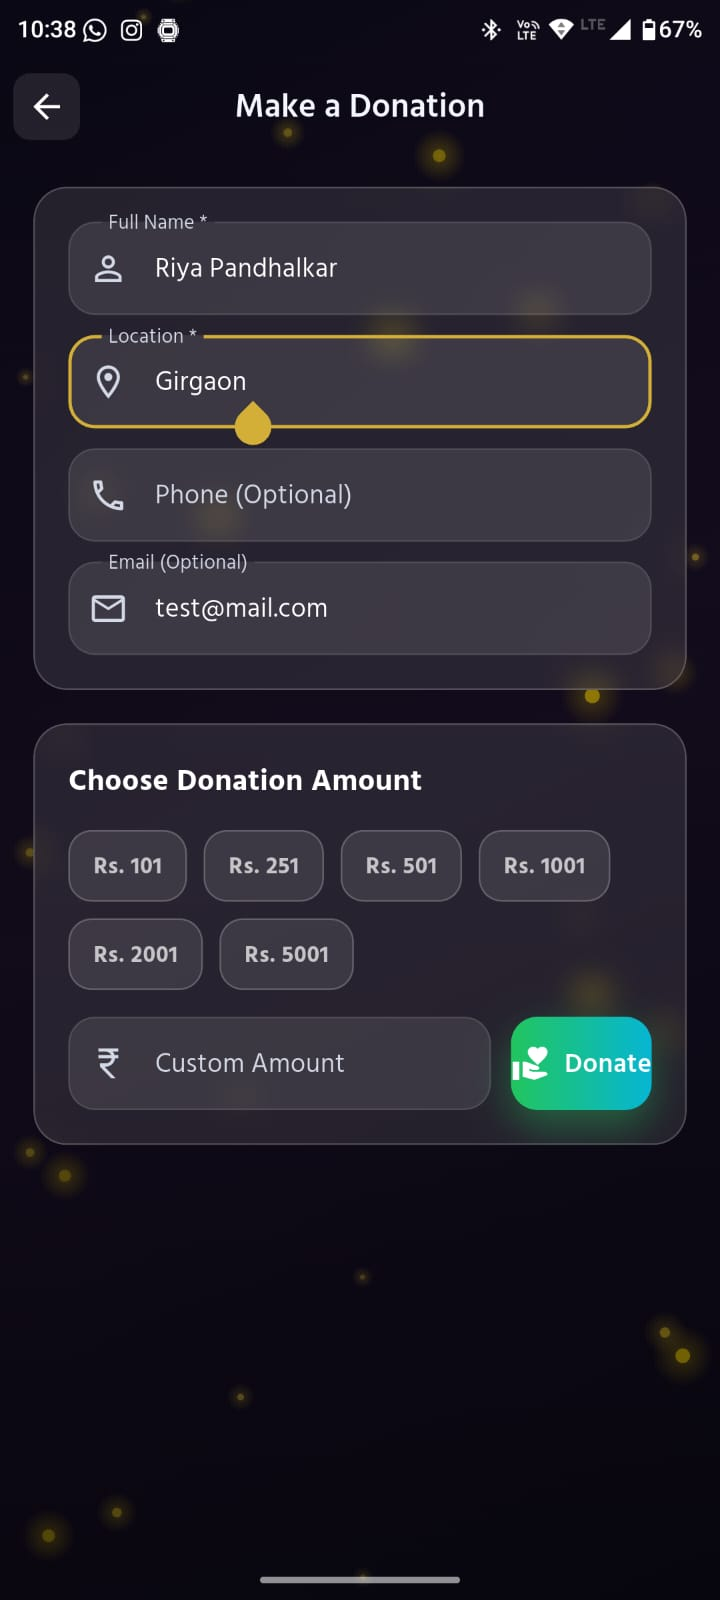
\includegraphics[width=0.32\textwidth]{images/donate_step1.jpg}
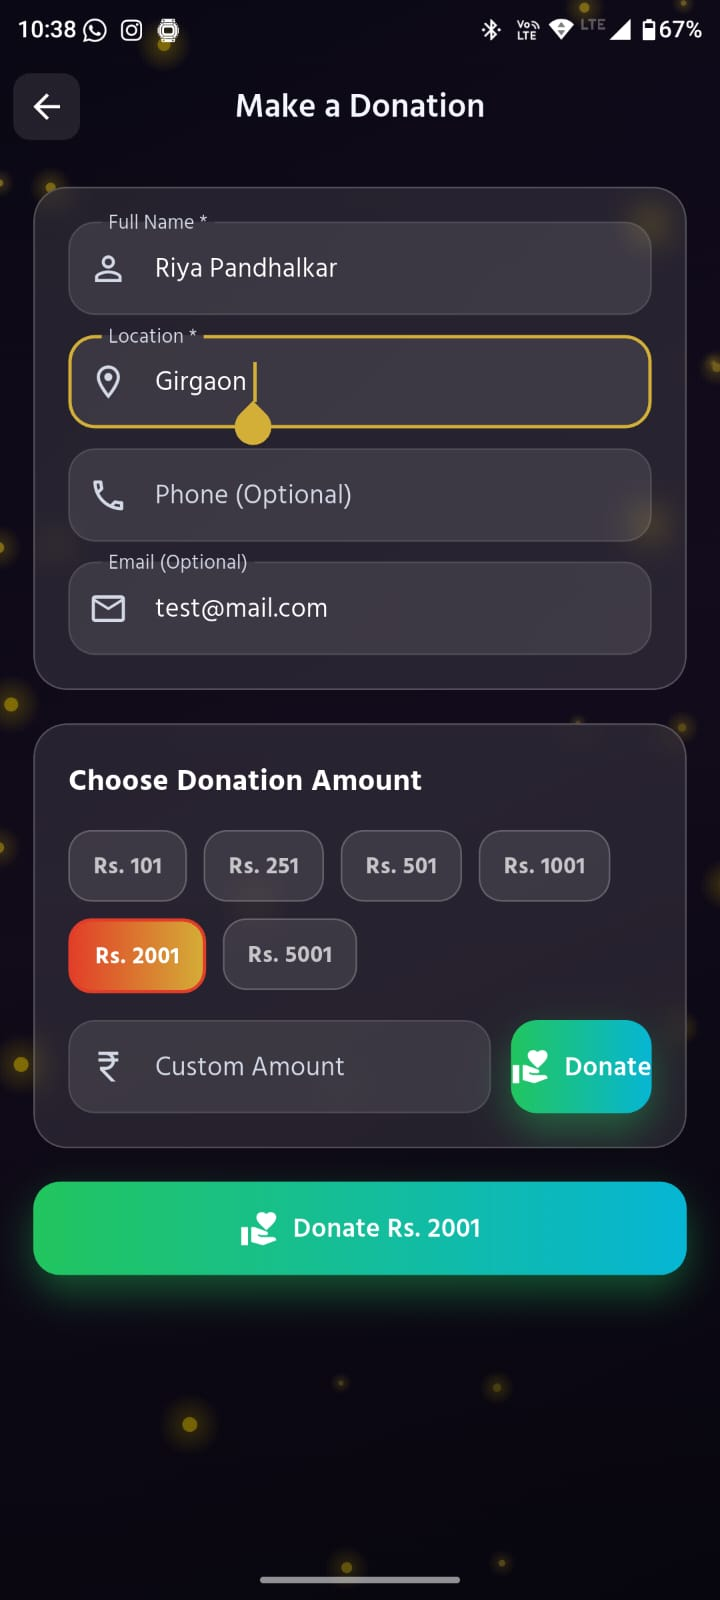
\includegraphics[width=0.32\textwidth]{images/donate_step2.jpg}
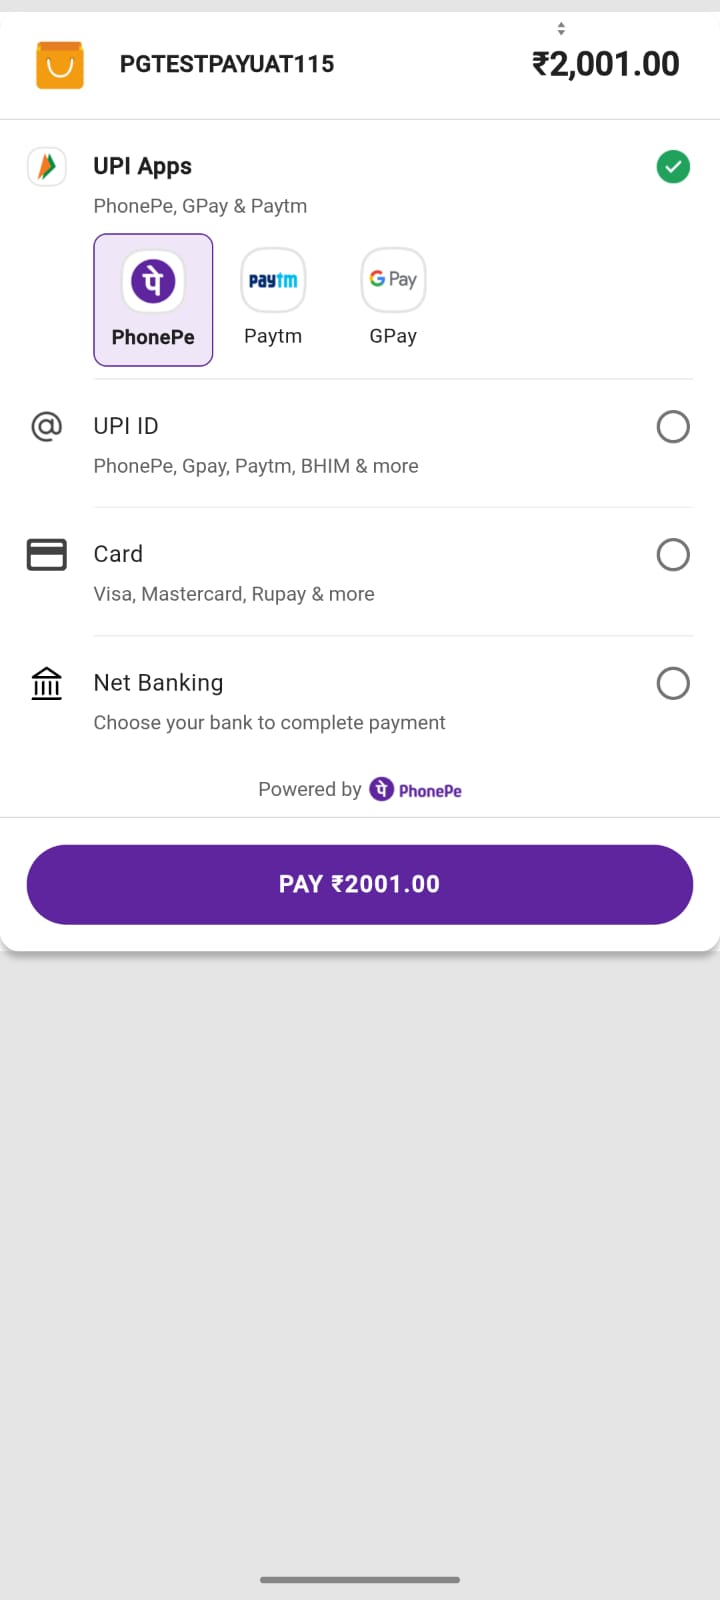
\includegraphics[width=0.32\textwidth]{images/donate_step3.jpg}
\caption{Four-step guided donation with progress indicator and celebratory success screen with confetti.}
\end{figure}

\subsection{6. Community \& Settings}
\begin{figure}[H]
\centering
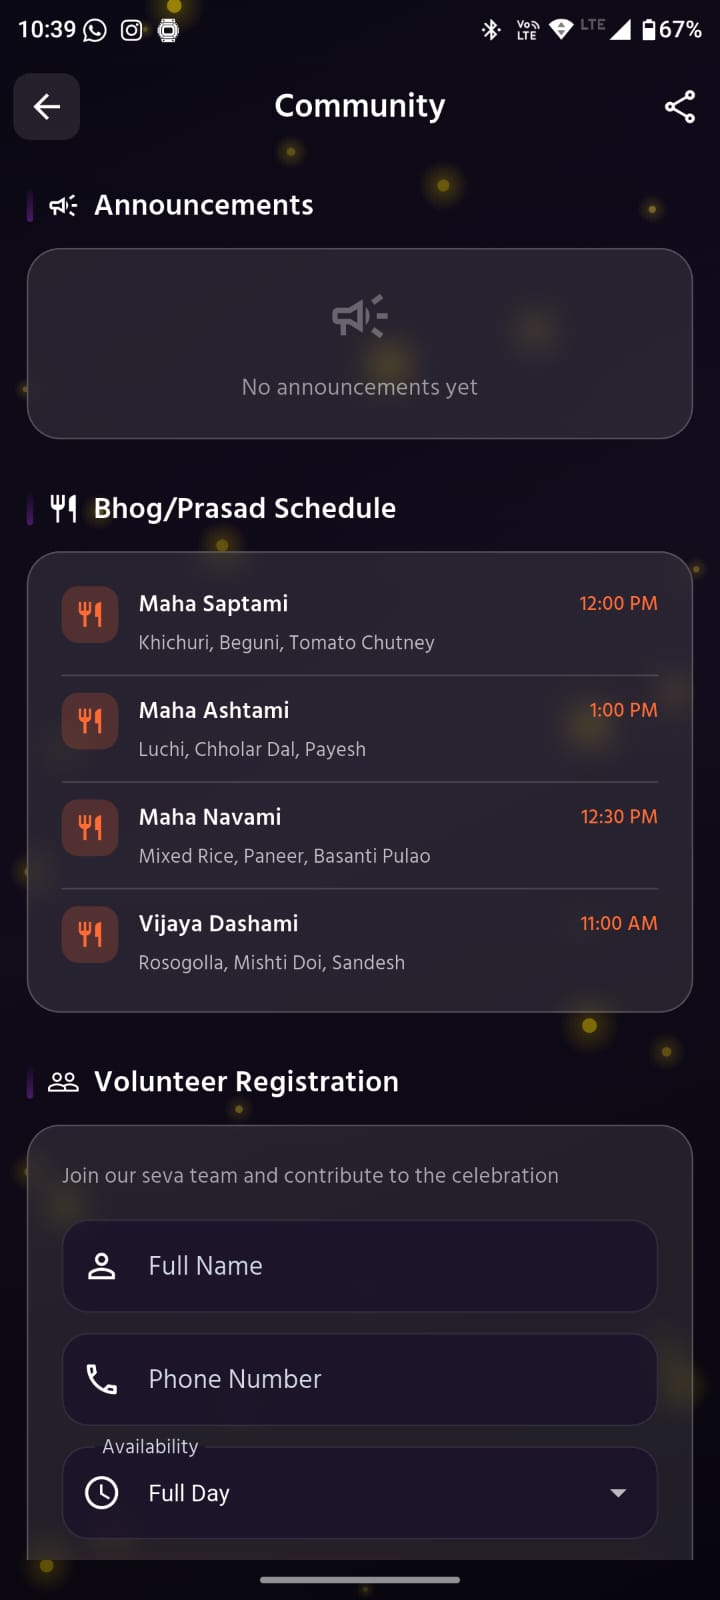
\includegraphics[width=0.48\textwidth]{images/community_feed.jpg}
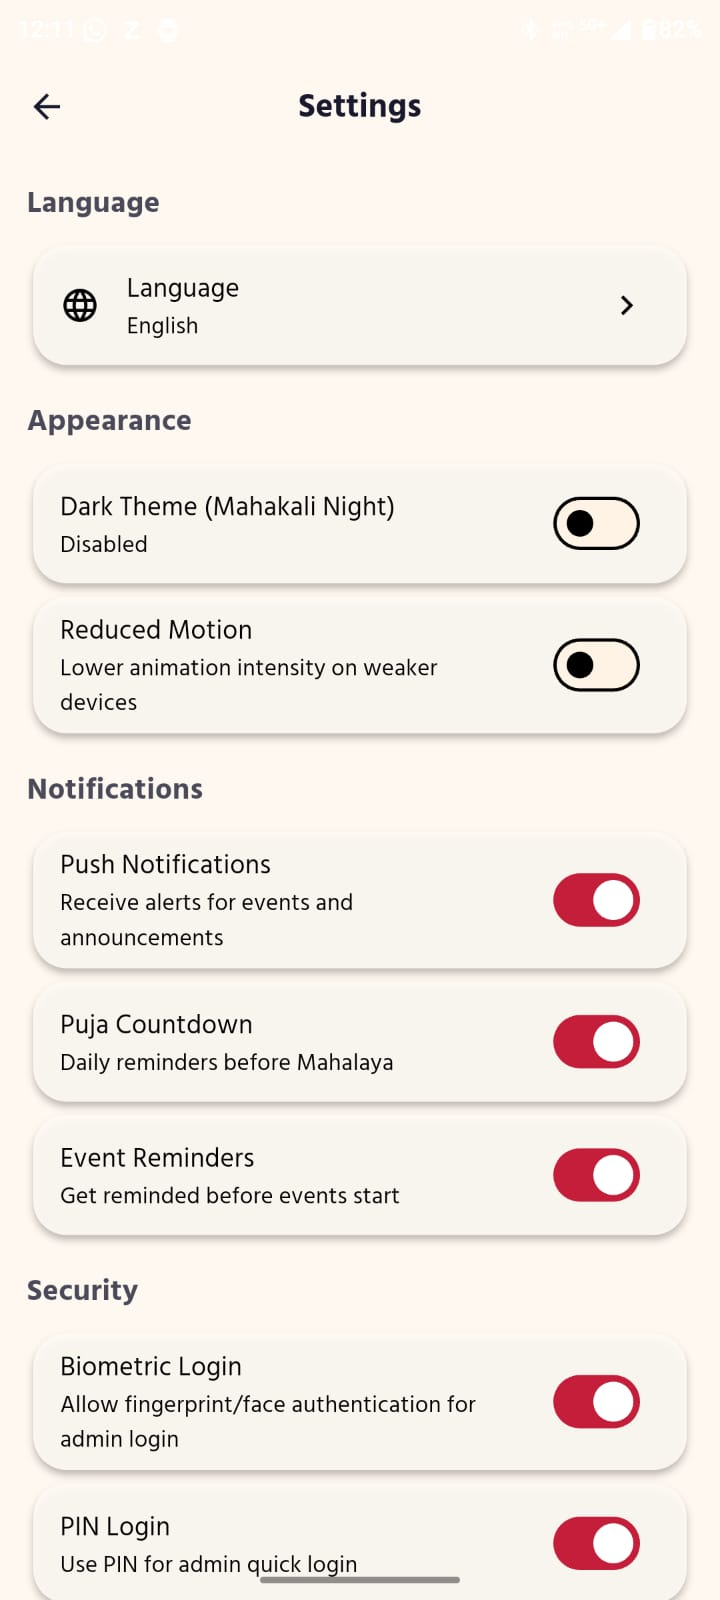
\includegraphics[width=0.48\textwidth]{images/setting_theme.jpg}
\caption{Real-time community feed and live theme switcher (Light/Dark/Festive modes).}
\end{figure}

\section{Design Process \& UI/UX Highlights}
\begin{itemize}
    \item \textbf{Research}: 3-day user interviews + competitive analysis of existing Puja apps.
    \item \textbf{Wireframing}: Low-fidelity in Figma → high-fidelity prototypes with 12 micro-interactions.
    \item \textbf{Color Theory}: Primary palette derived from traditional Durga Puja — \#B71C1C (deep red), \#FFD700 (gold), \#0D47A1 (deep blue).
    \item \textbf{Typography}: Playfair Display (headings) + Poppins (body) for perfect readability.
    \item \textbf{Motion Design}: 8 custom animations using Flutter’s AnimationController; Gooey effect via CustomPainter + bezier curves.
\end{itemize}

All decisions were validated through 5 usability testing rounds with target users.

\section{Challenges Faced \& Solutions}
\begin{itemize}
    \item Challenge: Creating liquid Gooey effect in Flutter → Solution: CustomPainter with animated bezier paths.
    \item Challenge: Offline-first gallery with large images → Solution: CachedNetworkImage + asset fallbacks.
    \item Challenge: Theme switching without reload → Solution: Provider + AnimatedTheme widget.
\end{itemize}

\section{Conclusion \& Future Roadmap}

\textbf{Impact}: This app has the potential to digitize and enhance Durga Puja celebrations for 10,000+ users in its first year.

\textbf{Future Improvements (Post-Hackathon)}
\begin{itemize}
    \item Real Razorpay/UPI integration
    \item AR/VR pandal preview using ARCore
    \item Admin panel for organizers (Flutter Web)
    \item AI-powered event recommendations
    \item Multi-city expansion + 10+ regional languages
    \item Blockchain-based transparent donation ledger
    \item Integration with Google Calendar \& Maps API
\end{itemize}

\textbf{Acknowledgments}
We express sincere gratitude to:
\begin{itemize}
    \item GDG On Campus SIESGST and Friends of Figma Mumbai for organizing PixelVerse 2026
    \item Flutter community and official documentation
    \item Durga Puja committees who shared cultural insights
    \item Our mentors and family for continuous support
\end{itemize}

This project truly embodies \textit{``Where Logic Meets Aesthetic''} — a functional masterpiece wrapped in cultural beauty.

We are excited to present this live during the offline round on \textbf{8 March 2026} at SIESGST, Nerul.
Thank you for your valuable time and consideration!




\end{document}